% This is "sig-alternate.tex" V2.0 May 2012
% This file should be compiled with V2.5 of "sig-alternate.cls" May 2012
%
% This example file demonstrates the use of the 'sig-alternate.cls'
% V2.5 LaTeX2e document class file. It is for those submitting
% articles to ACM Conference Proceedings WHO DO NOT WISH TO
% STRICTLY ADHERE TO THE SIGS (PUBS-BOARD-ENDORSED) STYLE.
% The 'sig-alternate.cls' file will produce a similar-looking,
% albeit, 'tighter' paper resulting in, invariably, fewer pages.
%
% ----------------------------------------------------------------------------------------------------------------
% This .tex file (and associated .cls V2.5) produces:
%       1) The Permission Statement
%       2) The Conference (location) Info information
%       3) The Copyright Line with ACM data
%       4) NO page numbers
%
% as against the acm_proc_article-sp.cls file which
% DOES NOT produce 1) thru' 3) above.
%
% Using 'sig-alternate.cls' you have control, however, from within
% the source .tex file, over both the CopyrightYear
% (defaulted to 200X) and the ACM Copyright Data
% (defaulted to X-XXXXX-XX-X/XX/XX).
% e.g.
% \CopyrightYear{2007} will cause 2007 to appear in the copyright line.
% \crdata{0-12345-67-8/90/12} will cause 0-12345-67-8/90/12 to appear in the copyright line.
%
% ---------------------------------------------------------------------------------------------------------------
% This .tex source is an example which *does* use
% the .bib file (from which the .bbl file % is produced).
% REMEMBER HOWEVER: After having produced the .bbl file,
% and prior to final submission, you *NEED* to 'insert'
% your .bbl file into your source .tex file so as to provide
% ONE 'self-contained' source file.
%
% ================= IF YOU HAVE QUESTIONS =======================
% Questions regarding the SIGS styles, SIGS policies and
% procedures, Conferences etc. should be sent to
% Adrienne Griscti (griscti@acm.org)
%
% Technical questions _only_ to
% Gerald Murray (murray@hq.acm.org)
% ===============================================================
%
% For tracking purposes - this is V2.0 - May 2012

%\documentclass{acm_proc_article-sp}
\documentclass{sig-alternate}
\usepackage{color}
\usepackage{multirow}
\usepackage{listings}
\usepackage{url}

\lstset{language=java, numbers=left, numberstyle=\tiny\color{black}, numbersep=3pt, escapeinside={\$}, basicstyle=\footnotesize\ttfamily, escapeinside={\%*}{*)}}

\newif\ifdraft
\drafttrue
%\draftfalse                                                                              
\ifdraft
\newcommand{\zhaonote}[1]{{\textcolor{cyan}    { ***Zhao:      #1 }}}
\newcommand{\note}[1]{ {\textcolor{red}    {\bf #1 }}}
\else
\newcommand{\zhaonote}[1]{}
\newcommand{\note}[1]{}
\fi


\begin{document}

\title{Gineala: Diagnosing Data with Machine Learning Pipeline Lineage}

\numberofauthors{3} 
\author{
% 1st. author
\alignauthor Zhao~Zhang\\\
       \affaddr{AMPLab}\\
       \affaddr{University of California, Berkeley} \\
       \email{zhangzhao@berkeley.edu}    
% 4th. author       
\alignauthor Evan~Sparks\\\
       \affaddr{AMPLab}\\
       \affaddr{University of California, Berkeley}\\
       \email{sparks@berkeley.edu}       
% 6th. author
\alignauthor Michael~J.~Franklin\\
       \affaddr{AMPLab}\\
       \affaddr{University of California, Berkeley}\\
       \email{franklin@berkeley.edu}   
}

\maketitle

\begin{abstract}
We present the Gineala lineage system as part of the KeystoneML machine learning pipeline to provide
users the capability of end-to-end data investigation. 
Practically, users can better understand the machine learning process and results with such analysis.
They can also possibly identify and remove data anomalies in the dataset, then replay the training or
prediction phase with clean data.
Gineala collects lineage at the transformer level by recording the computation itself, the mapping
between input and output elements, and optionally the input/output dataset along with a placeholder
for random factors. 
Gineala stores the lineage data on the underneath file system, and builds index over the lineage data
according to the lineage type. 
Among the four lineage types, the region lineage is often problematic, as storing and querying it with
native solution incurs unacceptable memory consumption and disk storage. 
We introduce a higher order function solution to describe region lineage, and investigate a number of indexing
algorithms to expedite queries. 
Experiments show that our higher order function solution reduce the storage overhead for region lineage 
by an oder of magnitude, and the indexing algorithms can speedup the random and batch query by 168x and 45x,
respectively.
We also present two use case studies of Gineala for image classification and astronomy object detection.
\end{abstract}

% A category with the (minimum) three required fields
\category{I}{Have}[No Idea]
%\keywords{ACM proceedings, \LaTeX, text tagging}

\section{Introduction}
Recording fine grained lineage information for modern distributed computing frameworks can help
users and practitioners understand the data analysis results, find data anomalies from massive
datasets, and replay the computation with cleaned data. 
Users can look into the lineage for a highly rated movie to understand the nature of the supporting
group. They can also investigate how an erroneous data item propagates in the analysis and replay
the computation by removing the polluted data at a stage that incurs the least re-execution cost.
In general, a lineage system needs to be able to collect the fine grained lineage, 
provide forward and backward query along the computation stages, and replay partial computation
that are of users' interest.

Building such a lineage system is particularly challenging because: 
1) lineage collection can slowdown the analysis dramatically;
2) lineage data can be hard to capture due to intermediate data's lack of structure;
3) lineage data can exceed the disk storage space; 
4) interaction between users and the lineage system needs to be responsive.

Specifically for a distributed machine learning system, some challenges can exacerbate: 
The slowdown introduced by recording lineage to disks can be significant as the computing engine 
may run applications completely in memory without writing/reading intermediate data to/from disks. 
The dataset processed by a distributed machine learning system is usually larger that runs on a desktop.
On the other hand, dedicated distributed machine learning systems have the intermediate data between
stages well structured as vectors, matrices, and images (2D images with channels). 
This allows us to separate the metadata of the coordination system in each data structure from the actual data. 
Recording the mapping between metadata and storing them consumes less storage space than that of actual data.
Building index for the metadata mapping can reduce the query response time while paying the cost of time.

In this paper, we investigate the above tradeoffs in the context of the KeystoneML machine learning pipeline that is built on
top of Apache Spark~\cite{zaharia12}. In particular, we study 1) various data storage options given a space or a query latency constraint, 
2) a set of indexing algorithms with different memory consumption, disk space, building overhead, and query latency.
Based on these studies, we present the Gineala lineage system as a module of KeytoneML. 
Gineala abstracts lineage as input dataset, output dataset, metadata mapping, computation, and random factor. 
Gineala lets users declare lineage in five pre-defined categories: {\bf One}, {\bf All}, {\bf Region}, {\bf LinCom} (Lineage Combination), and {\bf Gather}.
It separates the metadata (coordination system of the data structure) from the actual data, and records the metadata mapping. 
It incorporates metadata type checking for inter-stage lineage query and builds index for {\bf Region} lineage for responsive query.
Gineala stores lineage information in HDFS~\cite{shvachko10} as Apache Spark's resilient distributed dataset(RDD). 
It can load the lineage information into KeystoneML in-memory, modify or remove data item from the input dataset, and replay
the computation interactively.

The contributions of this paper are: 
1) the use of higher-order function to describe {\bf Region} lineage;
2) the indexing algorithm that speeds up the query by 45x-168x;
3) the open source implementation of the Gineala system.

We use three real machine learning pipelines to show Gineala's functionalities and performance. 
RandomFFTMNIST is a pipeline for hand-written digit recognition. 
VOCSIFTFisher is an image classification pipeline.
SourceExtractor is an astronomical image processing pipeline that detects objects in images produced by astronomy telescopes.
Our results show that by using the higher-order function for {\bf Region} lineage can reduce the the storage space by xxx. 
Indexing strategies with RTree and KMeans algorithms can speedup the query response time by a factor of xxx with overhead of xxx, respectively.
The overall slowdown for the three real pipelines are xxx, with xxx more memory and disk consupmtion.

The rest of the paper is organized as following: 
\S\ref{sec:Background} introduces the background of KeystoneML and typical uses of fine-grained lineage systems. 
\S\ref{sec:Lin} discusses lineage of a machine learning pipeline formally.
\S\ref{sec:Design} discusses the general design of Gineala.
\S\ref{sec:Impl} documents the Gineala implementation on KeystoneML with technical details
We present the performance measurements in \S\ref{sec:Perf}.
\S\ref{sec:Related} surveys existing lineage systems.
We conclude and envision future work in \S\ref{sec:Conclusion}.

\section{Background}
\label{sec:Background}
In this section, we briefly review the KeystoneML and introduces three use cases of Gineala.

\subsection{KeystoneML}
KeystoneML is an application framework designed for the implementation of robust large-scale machine learning pipelines. Built on the principles of declarative programming and modular design, KeystoneML provides a light-weight and elegant API that allows users to describe these pipelines as the composition of two types of operator--Transformers, which perform deterministic data transformation, and Estimators, which ``learn'' Transformers based on training data. KeystoneML pipelines are fit and executed in parallel using Apache Spark. These pipelines are compiled into an application DAG and optimized before execution. Current optimizations include online decisions about materialization of intermediate state, as well as standard optimizations such as common subexpression elimination. KeystoneML includes a library of standard feature extractors in domains including computer vision, audio, and text processing, as well as standard statistical procedures and Estimators for several types of machine learning model.

\subsection{Use Cases}
\subsubsection{Dense SIFT Features Visualization}

\subsubsection{Astronomy Image and Catalog Validation}

\subsubsection{Code Debugging}

\section{Lineage}
\label{sec:Lin}
In this section, we formally define the notion of pipeline, dataset, lineage and its associated operations of query and replay.

\subsection{Pipeline and Datasets}
\label{sec:Lin-Pipe-Data}
We define a dataset $I$ as a collection of structured data. In the scope of this work, the supported structures are: 
DenseVector, DenseMatrix, and Image. DenseVector is a one dimensional data structure and DenseVector is
two dimensional. Image is a three dimensional data structures that is defined by the height, the width and the number
of channels of an image. 

An element $e \in I$ has two properties: value $e.value$ and coordinates $e.coor$. 
Combining the additional dimension in the collection with the data structure, 
the coordinates of an element is a pair of integers, a triple of integers, or a quadruple of integers
for DenseVector, DenseMatrix, and Image, respectively.

A pipeline $P$ is defined as a sequence of transformers $(T_1, T_2, ..., T_n)$. 
Each transformer $T_i$ takes a dataset $I_i$ as its input, and produces $I_{(i+1)}$ as the output. 
Especially, we denote the output of the whole pipeline as $O = I_{n+1}$

\subsection{Dataset Companion}
Since transformers operate at the data structure (DenseVector, DenseMatrix, Image) level, we use the notation
$\overline{I_i(e)}$ as the companion of $I_i$ with respect to element $e$ such that $\forall a \in \overline{I_i(e)}$,
\[ a.value =
  \begin{cases}
    e.value       & \quad \text{if } a.coor = e.coor\\
    NaN  & \quad \text{otherwise}. \\
  \end{cases}
\]

Accordingly, given a list of distinct elements $(e_1, ..., e_m)$, the companion of $I_i$ with respect to $(e_1, ..., e_m)$ is
described as: $\forall a \in \overline{I_i(e_1, ..., e_m)}$, 
\[ a.value =
  \begin{cases}
    e.value       & \quad \text{if } \exists e \in (e_1,...,e_m), a.coor = e.coor\\
    NaN  & \quad \text{otherwise}. \\
  \end{cases}
\]


\subsection{Data Lineage and Replay}
Before defining the lineage, we need to introduce the relationship between the two data structures $A$ and $B$ with the same type.
We say $A \subseteq B \text{ or } B \supseteq A$, $\text{if }\forall a \in A, \exists b \in B, s.t.\text{ } a \neq NaN \land a.coor = b.coor \land a.value = b.value$.
By saying $A = B$, we mean $A \subseteq B \land B \subseteq A$.

We define the data lineage of a given element as the elements in the input dataset that is used to produce present element.
The single transformer lineage is
\begin{equation}
S(e \in I_{i+1}) = \{e_1, ..., e_m | T_i(\overline{I_i(e_1, ..., e_m)}) \supseteq \overline{I_{i+1}(e)}\}.
\label{equa:SingleLineage}
\end{equation}


Recursively, the lineage of a given element across multiple transformers can be defined as
\begin{equation}
L(e) = \cup_{e' \in S(e)} L(e').
\end{equation}

We define the property of $Replay(e \in I_{i+1}) = \overline{I_{i+1}(e)} \subseteq T_i(\overline{I_i(e_1, ..., e_m)})$ in Equation~\ref{equa:SingleLineage}
as the replay property, which means we can reproduce the output solely with its lineage and the corresponding transformer.
The constraint of the replay property is that only the element $e$ is guaranteed to be the same as the original transformation 1
if $\overline{I_{i+1}(e)} \subseteq T_i(\overline{I_i(e_1, ..., e_m)})$. In this case, the results of the replayed transformer may
produce inconsistent results for elements other than $e$ in $I_{i+1}$. 
In some cases, we see a stronger condition of $\overline{I_{i+1}(e)} = T_i(\overline{I_i(e_1, ..., e_m)})$, which indicates that
the replayed results are exactly the same as the original results.

The replay property for multiple elements require the lineage for all elements. Formally,
$Replay(e_1,..,e_m \in I_{i+1}) = \overline{I_{i+1}(e_1,...,e_m)} \subseteq \cup_{e \in (e_1,...,e_m)} Replay(e) $.

\subsection{Data Lineage Query}
The forward query of an element over data lineage of a pipeline $P$ returns $qForward(e) = \{e' | e \in L(e' \in O)\}$. 
And the backward query of an element over data lineage returns $qBackward(e) = e' \in L(e)$.
Specifically, the identifier of an element is its coordinates in the according data structure, so the query actually takes
the coordinates of the input element as key, and query over the data lineage. The query that spans multiple transformers 
use coordinates as intermediate data. Once the query reaches the final transformer, it associates the actual values
with the result element coordinates and return them.

Queries of multiple elements can then be expressed as the union of the query for each element: 
\begin{equation}
\begin{split}
qForward(e_1, ..., e_m) = \cup_{e \in (e_1, ..., e_m)} qForward(e) \\
qBackward(e_1, ..., e_m) = \cup_{e \in (e_1, ..., e_m)} qBackward(e).
\end{split}
\end{equation}

\section{Requirements}
\label{sec:Req}
The requirements of the Gineala lineage system for KeystoneML can be viewed from the functionality and performance perspective.

\subsection{Functional Requirements}
Gineala should expose a programming interface for users to declare and operate the lineage of each transformer. 
Gineala's built-in lineage should cover the most common lineage types and preserve the flexibility for users to declare their own lineage types.
Gineala also requires an interactive interface for users to load recorded lineage and query over it.

The single transformer lineage need to provide the forward query and backward query functionalities. 
It is  guaranteed that the lineage across transformers can be queried in a chain, as long as the transformers
can form a pipeline (the transformers' types conform the pipeline strong type checking).

The single transformer lineage should be able to be replayed deterministically, meaning that with the same input dataset and transformer,
the lineage can reproduce the identical result and the original result even with the presence of random factors.
In turn, a partial pipeline assembled by a sequence of transformers of the original pipeline should be able to be replayed deterministically.

\subsection{Performance Requirements}
\label{sec:Req-Perf}
As Gineala incurs additional computation and I/O to record and save lineage, the overall pipeline performance is expected to slowdown.
Especially for KeystoneML that is built upon Apache Spark, unlike other distributed computing framework such as Hadoop~\cite{HADOOP} 
that writes/reads intermediate data to disk, any additional I/O can introduce a more significant slowdown. 
The Hadoop-based lineage system Newt~\cite{logothetis13} reported a 20$\sim$50\% slowdown; 
another Hadoop-based lineage system GMRW~\cite{ikeda11} observed a slowdown of 16$\sim$76\% depending on the workloads;
the SciDB~\cite{brown10}-based SubZero~\cite{wu13} system introduced 50$\sim$150\% overhead. 
We expect Gineala's slowdown to the original pipeline to be comparable to these systems.

When Gineala records lineage, we face tradeoffs between performance slowdown, memory usage and disk space.
In some cases, it may run additional computations on the collected lineage to reduce the lineage size. 
E.g., regressing a sequence of coordinates to a higher order function. 
In other cases, it may cache all lineage information for a transformer before writing it to the storage. 
Gineala should be able to automatically instrument the lineage collection to adapt the constraints.

Lineage information can be massive depending on the transformer, since the input dataset or the intermediate dataset of a pipeline can be large.
In some transformers, the mapping between the input elements and output elements is complicated. 
Regress the element-wise mapping to a higher order function can reduce the storage overhead, however it introduce latency when users
query them. Thus Gineala requires indexing strategies for the recorded lineage to overcome this issue.

\section{Design}
\label{sec:Design}
Figure~\ref{fig:architecture} shows the overview of Gineala and its interactions with other components. 
Rounded-corner rectangles are components around and inside KeystoneML. 
The two-sided arrows indicate interactions between components.
Users compose machine learning pipelines with KeystoneML and submit the compiled DAG to Spark.
All computation and I/O are done through the Spark Resilient Distributed Dataset (RDD) abstraction.
With Gineala, users can declare and operate lineage at the transformer level, 
so that the compiled DAG also contains lineage recording and other operations, e.g., save to disk.
Lineage in Gineala is stored to HDFS~\cite{shvachko10} via Spark's RDD abstraction.
Users can load the stored lineage in HDFS to Spark interactive command line interface.
By calling Gineala primitives, users can query elements of interest, replay transformers, or analyze
the lineage for other purposes.

\begin{figure}[h]
\begin{center}
    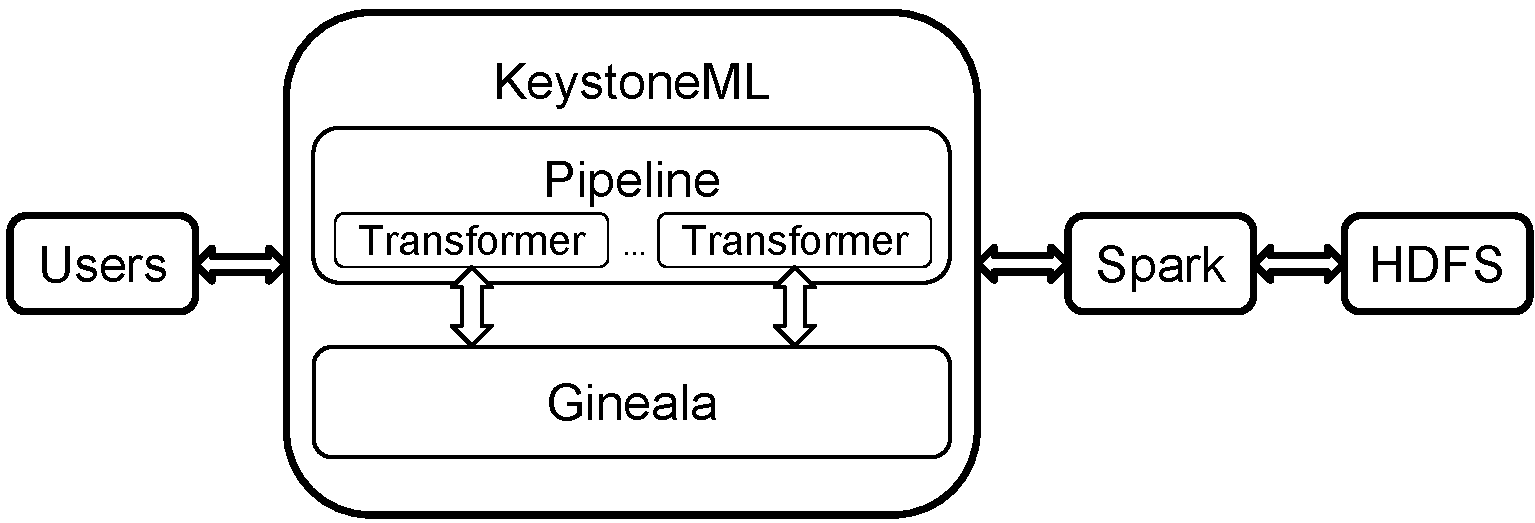
\includegraphics[width=85mm]{pictures/architecture}
\caption {Overview of Gineala and its surrounding components.
    \label{fig:architecture}
}
\end{center}
\end{figure}

\subsection{Lineage}
For each transformer, Gineala collects five types of data: the input dataset, the output dataset, the transformer, the collection of mapping, the model, and the random parameter.
The model stores the trained model of an estimator generated transformer.
The random parameter holds the information that guarantees the determinism of the transformer.

For estimators, we only consider linear model estimators in the current implementation. 
We view linear model estimators as transformers without model or random parameters, 
but instead we keep track of the training parameters that are used to obtain the output model (the output dataset). 

\subsection{Mapping}
Consider a transformer that transforms a RDD of matrices to another RDD of matrices.
A RDD of matrices can be understood as a distributed array of matrices that is distributed across a cluster.
We observe that many transformations in various pipelines has narrow dependencies, where a output matrix
only depends on one input matrix. Figure~\ref{fig:narrowmapping} shows this case. 
The left mapping is from an input RDD of matrices to an output RDD of matrices. 

\begin{figure}[h]
\begin{center}
    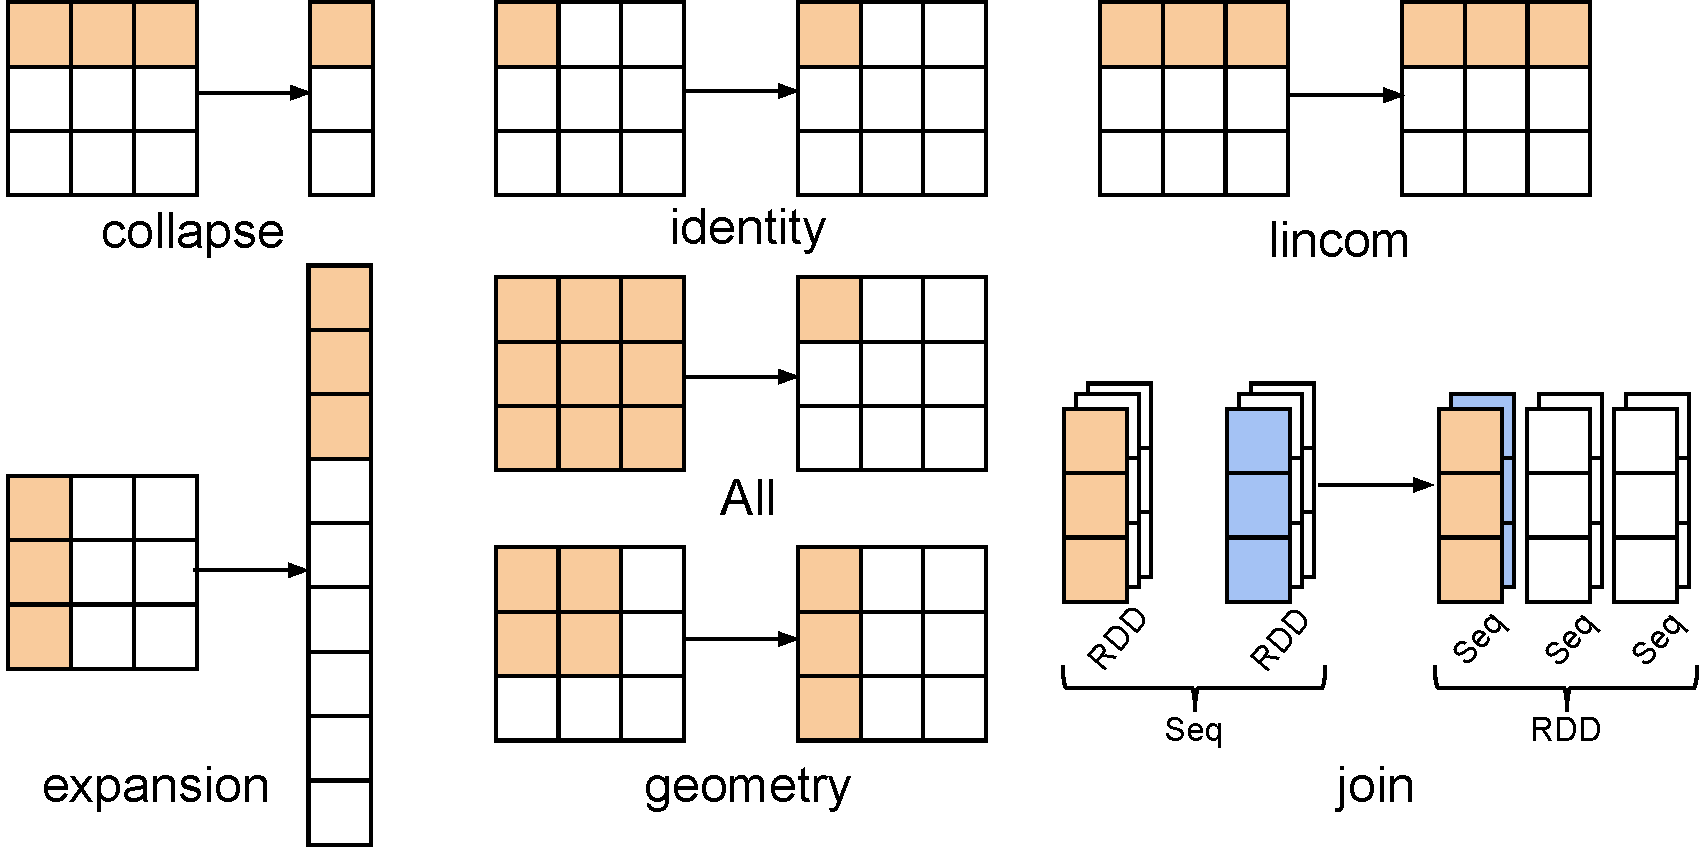
\includegraphics[width=85mm]{pictures/narrowmapping}
\caption {Left: The narrow mapping cases in the context of Resilient Distributed Dataset (RDD), rectangles are RDDS and rounded-corner rectangles are matrices.
Right: Three element-wise mapping cases, mappings are shown with color highlights.
    \label{fig:narrowmapping}
}
\end{center}
\end{figure}

Taking a pair of matrices and see the element-wise mapping, we see three types of mappings: 
{\bf One Mapping}, in which case each output element only depends on one element with the same coordinates in the input matrix.
{\bf All Mapping}, in which case each output element depends on all elements in the input matrix.
{\bf Region Mapping}, in which a group of output elements depend on a group of input elements.
{\bf Sample Mapping}, in which the output is a sample of the input.

In general, we also see the narrow dependencies and the three mapping cases in transformers with data structures of 
DenseVector and Images. 
So Gineala pre-defines these three element-wise mappings. 
In the next section, we will introduce how Gineala's lineage interface exposes the lineage declaration interface with the mapping information.

\zhaonote{saying One Mapping and All Mapping are symmetric.}

\subsection{Region Mapping}
As can be seen in the region mapping example in Figure~\ref{fig:narrowmapping}, the backward query of an output element should return all the input elements in the corresponding region. If the output region has $N$ elements and the input region has $N$ elements, the space complexity of storing such a mapping is $O(N^2)$. 
Inspired by the Scale-invariant feature transform (SIFT) and the SourceExtractor implementation, each of them processes an input matrix and produces thousands of vectors as outputs. An output vector depends on a group of elements in the matrix, and these elements form a two dimensional shape. 
For SIFT, the input elements form a circle with a geographical center and the scale as its radius.
Similarly, the SourceExtractor's input elements  form an ellipse. 
Gineala uses a higher-order function to describe the region. 
Thus the mapping between two regions is expressed as a tuple of two higher-order functions.
The space complexity goes down to O(1).

Since many softwares such as SIFT and SEP already return the geographical information with the results.
Gineala exposes some simple interfaces for two dimensional shapes as special cases.
Users can pass in the geographical information directly to declare square, circle, and ellipse.

Using the higher order function involves an issue for query. If the mapping is recorded at the element level, query is straight forward.
Given an output element, a backward query returns corresponding input elements.
Now both the input elements and output elements are encoded with a higher order function. 
And the mapping between input function and output function is stored in a list. 
A query that takes an output element as key thus needs to iterate over all input functions and test if the key is in the function or not.
If the key is in an input function, it then returns the mapping output function, and expands the function to a group of coordinates.
The time complexity of query over Region Mapping is then $O(N^2)$, assuming there are $N$ tuples in the list and each input function expands to $N$ elements.
To speedup the query performance, we implement and compare several indexing strategies, and a detailed discussion is in \S\ref{sec:RegionIndex}.

\subsection{Lineage Type}
Gineala defines three lineage interfaces at high level: NarrowLineage, GatherLineage, LinComLineage. 
NarrowLineage covers the lineage that has a narrow dependency and GatherLineage covers the dependency in a gather pattern, where the transformer takes a sequence of RDD of data structures and transform them into a single RDD of data structures. 
LinComLineage is for the transformer which is the output of fitting training dataset to the linear model estimator.

The NarrowLineage can then be further specified with a specific mapping pattern. E.g., NarrowLineage that has One Mapping is named as OneLineage.
For OneLineage and AllLineage, the users only need to pass the input dataset, output dataset, and the parameters, since Gineala can figure out the element-wise mapping from the metadata of the internal data structure.

For RegionLineage and SampleLineage, Gineala requires the mapping collection for the declaration. 
Such a collection should be a RDD of tuple list. 
Each tuple is a pair of the input region and the output region.

The GatherLineage is implemented within the GatherTransformer.
And so is LinComLineage for the linear model estimator. LinComLineage requires the model as input for declaration.
Both these two lineage types can adapt to DenseVectors, DenseMatrix, and Images. 
Users do not have to modify these two lineage types. 

\section{Implementations}
\label{sec:Impl}
This section discusses implementation details for lineage collection, I/O, and region mapping index.

\subsection{Metadata Separation}
\zhaonote{show a profile study of metadata size and actual data size, saying why metadata is mandatory, input/output datasets are optional}
As discussed in \S\ref{sec:Req-Perf}, writing lineage to persistent storage can introduce a more dramatical slowdown for KeystoneML comparing
to the Hadoop-based systems, since Spark seeks to eliminate unnecessary I/O between memory and persistent storage.
One effective way to reduce the I/O overhead is reduce the lineage data size.

Gineala reduces the lineage data size by 1) separating the metadata from the datasets, 2) tracking only the metadata mapping, 
3) taking advantage of the mapping types specified by the user, 4) and writing datasets to persistent storage with a configurable 
setting in the lineage instrumentation in the transformer.

In \S\ref{sec:Lin-Pipe-Data}, we say an element in a data structure has two properties: the coordinate and the value.
We refer the coordinate as the metadata of a particular element and the value as the actual data. 
In a backward query of an element throughout the whole pipeline, the query traverses from the last transformer
to the very first transformer in a sequential manner. 
We see that in the last the transformer and other transformers in the middle, the metadata mapping is sufficient to answer
the query of depending input elements of given output elements. Only in the very first transformer do we need both the metadata
to find the metadata of the depending input elements and the actual data of these elements.
So Gineala separates the metadata from actual data and only tracks the metadata mapping.

Another lineage size reduction is contributed by user specified mapping types. 
For the lineage type of {\em OneLineage} and {\em AllLineage}, it is simple for Gineala to infer the mapping from the
metadata of the data structure. E.g., the height and width of a matrix. 
In these case, Gineala only records the data structure metadata instead of individual mapping tuple.
Similar approaches can be applied for {\em GatherLineage} and {\em LinComLineage}.
While for {\em SampleLineage} and {\em RegionLineage}, the mapping is between two groups of elements, thus it is
not feasible to use data structure metadata to infer the mapping.

A profile study of the VOCSIFTFisher pipeline shows that the actual data size is 840.9~GB and the metadata size
is 61.3~GB. Writing only metadata can reduce the total I/O amount by a factor of 13.7x.

For the actual data, Gineala only stores the input dataset for the very beginning transformer as mandatory. 
Users can configure the Gineala to make decisions for other transformers' input and output datasets.




\subsection{Lineage I/O}
\zhaonote{what data to store}
Among these five data types, the transformer and the collection of mapping are mandatory. 
The input dataset is mandatory if the transformer is the very first of the pipeline. 
Otherwise, the input dataset is optional.
The output dataset is optional, as it can be reproduced by rerunning the transformer with the input dataset.
\zhaonote{save to HDFS thorugh RDD abstraction, file path consistent with transformer nametag and the very original input RDD id}

\subsection{Region Mapping Index}
\label{sec:RegionIndex}
\zhaonote{Direct, RTree, Kmeans}

\subsection{Replay}
\zhaonote{replay single transformer and multiple transformers}

\section{Performance Measurements}
\label{sec:Perf}
Measurements

\subsection{Overhead}
Overhead

\subsection{Query}
Query

\subsection{Replay}
Replay

\subsection{Use Case}
Query

\section{Related Work}
\label{sec:Related}
Related work

\section{Conclusion and Future Work}
\label{sec:Conclusion}
Conclusion

%ACKNOWLEDGMENTS are optional
\section{Acknowledgments}
This research is supported in part by NSF CISE Expeditions Award CCF-1139158, LBNL Award 7076018, and DARPA XData Award FA8750-12-2-0331, and gifts from Amazon Web Services, Google, SAP,  The Thomas and Stacey Siebel Foundation, Adatao, Adobe, Apple, Inc., Blue Goji, Bosch, C3Energy, Cisco, Cray, Cloudera, EMC, Ericsson, Facebook, Guavus, Huawei, Intel, Microsoft, NetApp, Pivotal, Samsung, Splunk, Virdata, VMware, and Yahoo!. 

%
% The following two commands are all you need in the
% initial runs of your .tex file to
% produce the bibliography for the citations in your paper.
\bibliographystyle{abbrv}
\bibliography{Lineage} % sigproc.bib is the name of the Bibliography in this case
% You must have a proper ".bib" file
%  and remember to run:
% latex bibtex latex latex
% to resolve all references
%
% ACM needs 'a single self-contained file'!
%
%APPENDICES are optional
%\balancecolumns



\balancecolumns

% That's all folks!
\end{document}
